\documentclass[border=10pt]{standalone}
\usepackage{tikz}
\usetikzlibrary{arrows.meta,shapes,calc,positioning}

\begin{document}
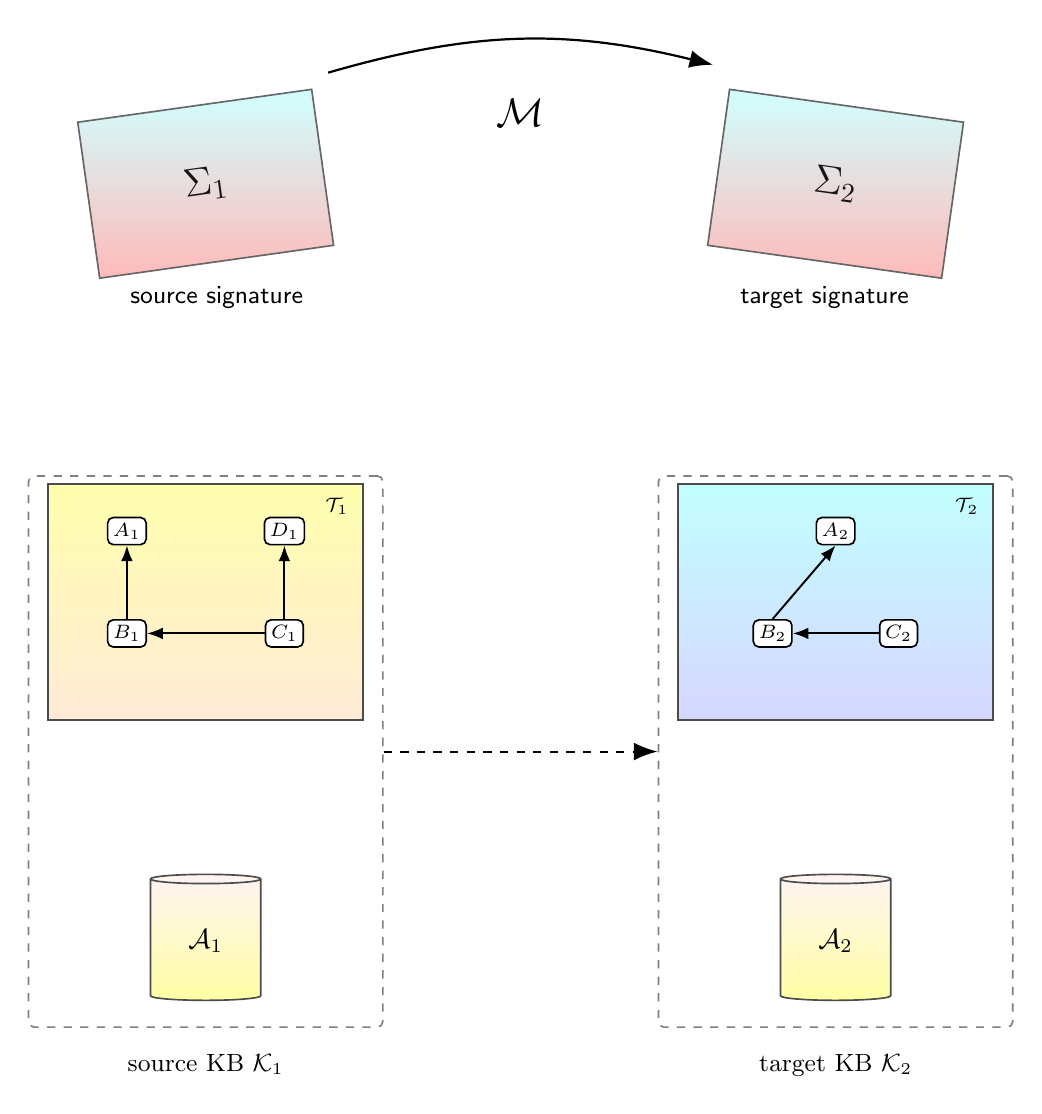
\begin{tikzpicture}[font=\sffamily,
    node distance=1cm,
    >=Latex,
    every path/.style={line width=0.6pt}
]

% Styles
\tikzset{
  sigrect/.style={
    rectangle,
    minimum width=3cm,
    minimum height=2cm,
    draw=black!60,
    top color=cyan!20,
    bottom color=red!30,
    fill opacity=0.9
  },
  tbox/.style={
    rectangle,
    minimum width=4cm,
    minimum height=3cm,
    draw=black!70,
    top color=yellow!40,
    bottom color=orange!20,
    fill opacity=0.8
  },
  tboxR/.style={
    rectangle,
    minimum width=4cm,
    minimum height=3cm,
    draw=black!70,
    top color=cyan!30,
    bottom color=blue!20,
    fill opacity=0.8
  },
  dashedframe/.style={
    rectangle,
    rounded corners=2pt,
    draw=black!50,
    dashed,
    inner sep=4pt,
    minimum width=4.5cm,
    minimum height=7cm
  },
  concept/.style={
    rectangle,
    rounded corners=2pt,
    draw=black,
    fill=white,
    inner sep=2pt,
    font=\scriptsize
  },
  cyl/.style={
    cylinder,
    draw=black!70,
    aspect=0.5,
    shape border rotate=90,
    minimum height=1.6cm,
    minimum width=1.4cm,
    top color=pink!20,
    bottom color=yellow!40,
    fill opacity=0.9
  }
}

%--------------------------------
% Top signatures
%--------------------------------

% Coordinates for top rectangles
\coordinate (S1) at (-4,3.5);
\coordinate (S2) at (4,3.5);

\node[sigrect,transform shape,rotate=8,anchor=center] (Sig1) at (S1)
   {\Large$\Sigma_{1}$};
\node[sigrect,transform shape,rotate=-8,anchor=center] (Sig2) at (S2)
   {\Large$\Sigma_{2}$};

% Curved arrow between signatures
\draw[-{Latex[length=3mm]},line width=0.8pt]
  ($(Sig1.north east)+(0.2,0.2)$)
    to[bend left=15]
  ($(Sig2.north west)+(-0.2,0.3)$);

% Label M on arrow
\node[font=\Large,above] at (0,4.1) {$\mathcal{M}$};

% text under signatures
\node[below=5pt of Sig1] {\small source signature};
\node[below=5pt of Sig2] {\small target signature};

%--------------------------------
% Bottom big dashed frames
%--------------------------------

\node[dashedframe,anchor=north] (FrameL) at (-4,-0.2) {};
\node[dashedframe,anchor=north] (FrameR) at (4,-0.2) {};

%--------------------------------
% TBoxes inside frames
%--------------------------------

\node[tbox,anchor=north] (T1) at ($(FrameL.north)+(0,-0.1)$) {};

\node[tboxR,anchor=north] (T2) at ($(FrameR.north)+(0,-0.1)$) {};

% TBox labels
\node[anchor=north east,font=\scriptsize] at ($(T1.north east)+(-2pt,-2pt)$) {$\mathcal{T}_{1}$};
\node[anchor=north east,font=\scriptsize] at ($(T2.north east)+(-2pt,-2pt)$) {$\mathcal{T}_{2}$};

%--------------------------------
% Concepts and arrows in T1
%--------------------------------

\node[concept] (A1) at ($(T1.center)+(-1,0.9)$) {$A_{1}$};
\node[concept] (B1) at ($(T1.center)+(-1,-0.4)$) {$B_{1}$};
\node[concept] (C1) at ($(T1.center)+(1,-0.4)$) {$C_{1}$};
\node[concept] (D1) at ($(T1.center)+(1,0.9)$) {$D_{1}$};

\draw[-{Latex[length=2mm]},line width=0.7pt]
   (B1.north) -- (A1.south);
\draw[-{Latex[length=2mm]},line width=0.7pt]
   (C1.north) -- (D1.south);
\draw[-{Latex[length=2mm]},line width=0.7pt]
   (C1.west) -- (B1.east);

%--------------------------------
% Concepts and arrows in T2
%--------------------------------

\node[concept] (A2) at ($(T2.center)+(0,0.9)$) {$A_{2}$};
\node[concept] (B2) at ($(T2.center)+(-0.8,-0.4)$) {$B_{2}$};
\node[concept] (C2) at ($(T2.center)+(0.8,-0.4)$) {$C_{2}$};

\draw[-{Latex[length=2mm]},line width=0.7pt]
   (C2.west) -- (B2.east);
\draw[-{Latex[length=2mm]},line width=0.7pt]
   (B2.north) -- (A2.south);

%--------------------------------
% Cylinders (ABoxes)
%--------------------------------

\node[cyl] (AB1) at ($(FrameL.south)+(0,1.1)$) {};
\node[cyl] (AB2) at ($(FrameR.south)+(0,1.1)$) {};
\node at (AB1.center) {$\mathcal{A}_{1}$};
\node at (AB2.center) {$\mathcal{A}_{2}$};

% Labels under frames
\node[below=6pt,font=\small] at (FrameL.south) {source KB $\mathcal{K}_{1}$};
\node[below=6pt,font=\small] at (FrameR.south) {target KB $\mathcal{K}_{2}$};

% Dashed arrow between frames
\draw[dashed,-{Latex[length=3mm]},line width=0.7pt]
  ($(FrameL.east)+(0,0)$) -- ($(FrameR.west)+(0,0)$);

\end{tikzpicture}
\end{document}